\chapter{Backend Simulators}


PICSimLab currently supports five backend simulators:
\href{https://github.com/lcgamboa/picsim}{picsim},  
\href{https://github.com/buserror/simavr}{simavr}, 
\href{http://mazsola.iit.uni-miskolc.hu/\%7edrdani/embedded/ucsim/}{uCsim}, 
\href{http://gpsim.sourceforge.net/}{gpsim} and 
qemu (\href{https://beckus.github.io/qemu_stm32/}{stm32} and \href{https://github.com/a159x36/qemu}{esp32}).


The type of debug interface depends on the backend simulator utilized.

\section{PICsim} \hypertarget{def:PICSim}{}

``\href{https://github.com/lcgamboa/picsim}{PICsim} emulates some PIC microcontroller and periferics such as USART and timers, the simulator architecture permit easy implementation of external elements in c language. It can be used as a standalone simulator (picsim executable) or as a library in other programs (As in PICSimLab).''


\subsection{MPLABX Integrated Debug } \hypertarget{def:mplabxd}{}

To use the \href{http://www.microchip.com/mplabx}{MPLABX} IDE for debug and program the PicsimLab, install the plugin \href{https://github.com/lcgamboa/picsimlab_md/releases/}{com-picsim-picsimlab.nbm} in MPLABX.

The plugin connect to PICSimLab through a TCP socket using port 1234 (or other defined in configuration window), and you have to allow the access in the firewall.

\href{https://lcgamboa.github.io/picsimlab_docs/stable/UsewithMPLABX.html}{Tutorial: how to use MPLABX to program and debug PICsimLab}.


\section{simavr}\hypertarget{def:simavr}{}

``\href{https://github.com/buserror/simavr}{simavr} is a new AVR simulator for linux, or any platform that uses avr-gcc. It uses avr-gcc's own register definition to simplify creating new targets for supported AVR devices. The core was made to be small and compact, and hackable so allow quick prototyping of an AVR project. The AVR core is now stable for use with parts with <= 128KB flash, and with preliminary support for the bigger parts. The simulator loads ELF files directly, and there is even a way to specify simulation parameters directly in the emulated code using an .elf section. You can also load multipart HEX files.''

\subsection{avr-gdb Debug} \hypertarget{def:gdbavr}{}
 
 With debug support enabled you can use avr-gdb to debug the code used in the simulator. 
 Use the configuration window to choose between MDB (MPLABX) or GDB to debug AVR microcontrollers. 
 
 
 Use avr-gdb with the .elf file as the parameter:
 \begin{verbatim}
 avr-gdb compiled_file.elf
 \end{verbatim}
 and the command below to connect (1234 is the default port):
 \begin{verbatim}
 target remote localhost:1234
 \end{verbatim}

Graphic debug mode can be made using \href{https://www.eclipse.org/}{eclipse IDE} with \href{https://eclipse.baeyens.it/}{Sloeber Arduino plugin}.

It is also possible to debug using \href{https://platformio.org/}{platformIO in VSCode}, just add the configuration lines below in the project's \textbf{platformio.ini} file:
\begin{verbatim}
;upload_protocol = arduino
;upload_port = COM7
;upload_port = /dev/tnt3
;monitor_port = /dev/tnt3

upload_protocol = custom
upload_command = C:\"Program Files"\PicsimLab\picsimlab_tool.exe loadhex "$BUILD_DIR/firmware.hex"
;upload_command = /usr/bin/picsimlab_tool loadhex "$BUILD_DIR/firmware.hex"

build_type = debug
debug_tool = custom
debug_port = localhost:1234
debug_build_flags = -O2 -g
debug_init_break = tbreak setup
debug_init_cmds =
  define pio_reset_halt_target
  end
  define pio_reset_run_target
  end
  target extended-remote $DEBUG_PORT
  $LOAD_CMDS
  pio_reset_halt_target
  $INIT_BREAK
\end{verbatim}
%Compile, and upload the code to PICSimLab before starting Debug.

\subsection{MPLABX Int. Debug }
PICSimLab also supports using MPLABX to debug simavr. The configuration is the same as described in PICSim section: \hyperlink{def:mplabxd}{MPLABX Integrated Debug}. 
It's possible import and debug a Arduino sketch into MPLABX using the \href{https://github.com/janegilruud/chipKIT-importer-2.0}{Arduino import plugin}.

 \section{qemu-stm32} \hypertarget{def:qemu-stm32}{}
 ``\href{http://beckus.github.io/qemu_stm32/}{Qemu STM32}: QEMU with an STM32 microcontroller implementation''
 
 \subsection{arm-gdb Debug} \hypertarget{def:gdbarm}{}
 
 With debug support enabled you can use arm-none-eabi-gdb (or gdb-multiarch) to debug the code used in the simulator. 
 
 Use arm-none-eabi-gdb with the .elf file as the parameter:
 \begin{verbatim}
 arm-none-eabi-gdb compiled_file.elf
 \end{verbatim}
 and the command below to connect (1234 is the default port):
 \begin{verbatim}
 target extended-remote localhost:1234
 \end{verbatim}

Graphic debug mode can be made using \href{https://www.eclipse.org/}{eclipse IDE} with 
\href{https://projects.eclipse.org/projects/iot.embed-cdt}{Eclipse Embedded CDT} or using \href{https://platformio.org/}{platformIO in VSCode}, just add the configuration lines below in the project's \textbf{platformio.ini} file:
\begin{verbatim}
upload_protocol = custom
upload_command = C:\"Program Files"\PicsimLab\picsimlab_tool.exe loadbin "$BUILD_DIR/firmware.bin"
;upload_command = /usr/bin/picsimlab_tool loadbin "$BUILD_DIR/firmware.bin"

build_type = debug
debug_tool = custom
debug_port = localhost:1234
debug_build_flags = -O2 -g
debug_init_break = tbreak main
debug_init_cmds =
  define pio_reset_halt_target
      monitor system_reset
  end
  define pio_reset_run_target
      monitor system_reset
  end
  target extended-remote $DEBUG_PORT
  $LOAD_CMDS
  pio_reset_halt_target
  $INIT_BREAK
\end{verbatim}

It's possible to configure STM32CubeIDE to connect and debug using PICSimLab:

\begin{figure}[H]
\center
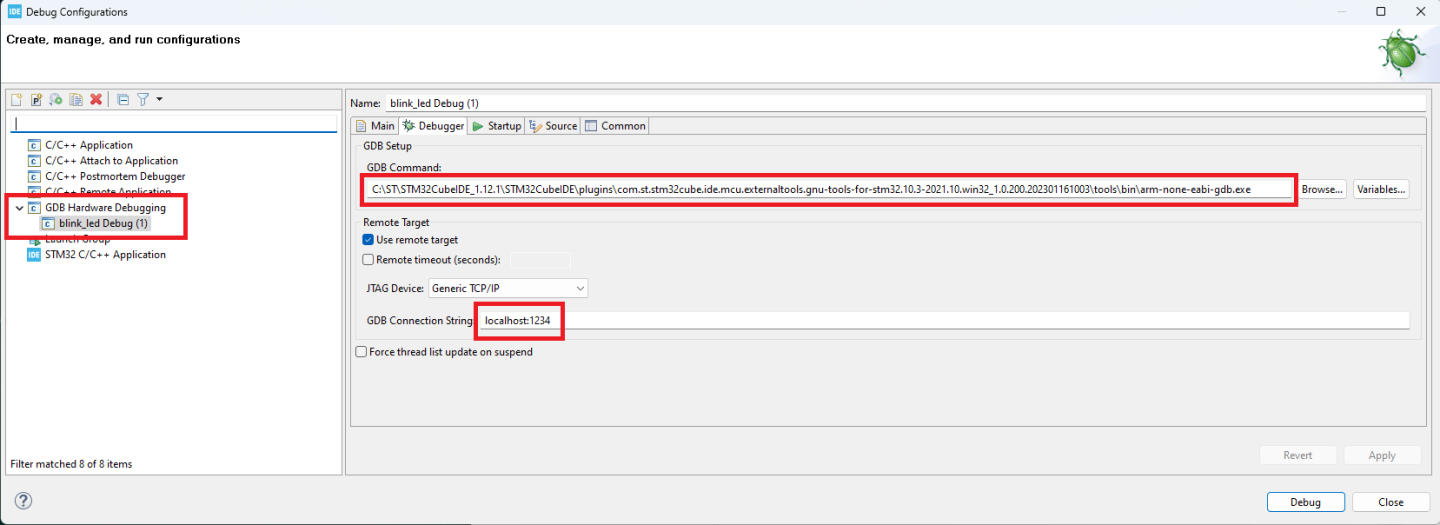
\includegraphics[width=0.99\textwidth]{img/configcube.png} 
\end{figure} 

\section{qemu-ESP32} \hypertarget{def:qemu-esp32}{}
 ``\href{https://github.com/a159x36/qemu}{Qemu ESP32}: Qemu Emulator for TTGO TDisplay esp32 board. ''
  
For integrated use with the Arduino IDE or IDF esptool.py , simply configure the serial port as explained 
in the Chapter \hyperlink{def:seriali}{Serial Communication} to flash PICSimLab ESP32-DevKitC as a real ESP32 board.

 \textcolor{red}{Atention!} Qemu ESP32 don´t support the QIO and QOUT flash modes, use only DIO or DOUT flash modes. 
 
\subsection{ESP32-gdb Debug} \hypertarget{def:gdbesp}{}

 With debug support enabled you can use xtensa-esp32-elf-gdb to debug the code used in the simulator. 
 
 Use xtensa-esp32-elf-gdb with the .elf file as the parameter:
 \begin{verbatim}
 xtensa-esp32-elf-gdb compiled_file.elf
 \end{verbatim}
 and the command below to connect (1234 is the default port):
 \begin{verbatim}
 target extended-remote localhost:1234
 \end{verbatim}

Graphic debug mode can be made using \href{https://platformio.org/}{platformIO in VSCode}, just add the configuration lines below in the project's \textbf{platformio.ini} file:
\begin{verbatim}
;upload_protocol = esptool
;upload_port = COM7
;upload_port = /dev/tnt2

upload_protocol = custom
upload_command = C:\"Program Files"\PicsimLab\picsimlab_tool.exe loadbin "$BUILD_DIR/firmware.bin"
;upload_command = /usr/bin/picsimlab_tool loadbin "$BUILD_DIR/firmware.bin"

build_type = debug
debug_tool = custom
debug_port = localhost:1234
debug_build_flags = -O2 -g
debug_init_break = tbreak main
debug_init_cmds =
  define pio_reset_halt_target
      monitor system_reset
  end
  define pio_reset_run_target
      monitor system_reset
  end
  target extended-remote $DEBUG_PORT
  $LOAD_CMDS
  pio_reset_halt_target
  $INIT_BREAK
\end{verbatim}

Compile, and upload the code to PICSimLab before starting Debug.
 
 
\section{uCsim} \hypertarget{def:ucsim}{}
``\href{http://mazsola.iit.uni-miskolc.hu/\%7edrdani/embedded/ucsim/}{uCsim} Software simulator for microcontrollers. uCsim can be used to simulate microcontrollers. It supports MCS51 family, AVR core, Z80, HC08, ST7, STM8, TLCS90, XA51 and Padauk. It can run on Linux, Windows, OSX, BSD, and other systems.''

\subsection{uCsim Debug} \hypertarget{def:ucsimdbg}{}
  
The uCsim debug console can be accessed with the telnet (1234 is the default port):
 \begin{verbatim}
 telnet localhost 1234
 \end{verbatim}
 
All \href{http://mazsola.iit.uni-miskolc.hu/\%7edrdani/embedded/ucsim/cmd.html}{uCsim commands} are supported.  

For windows users \href{https://www.putty.org/}{putty telnet client} is a good option to access the uCsim console. 
 
  
\section{gpsim} \hypertarget{def:gpsim}{}

``\href{http://gpsim.sourceforge.net/}{gpsim} is a full-featured software simulator for Microchip PIC microcontrollers distributed under the GNU General Public License, Version 2 or higher, and some of it's libraries under GNU Lesser General Public License, Version 2 or higher.

gpsim has been designed to be as accurate as possible. Accuracy includes the entire PIC - from the core to the I/O pins and including ALL of the internal peripherals. Thus it's possible to create stimuli and tie them to the I/O pins and test the PIC the same PIC the same way you would in the real world.'' 
  
  
\section{Remote} \hypertarget{def:remote}{}

This is experimental support to allow other simulators acting as microcontrollers to control PICSimLab remotely (TCP/IP).
